\section{Experiments}
\label{sec:experiments}

We evaluate two claims separately. The budget experiments ask whether an information-weighted policy family can meet an expected sensing-usage target, transfer that calibration across reward scales, and re-adapt after a scale change. The EFE experiments ask where the canonical $w{=}1$ policy lies relative to reward-only planning, tuned information gain, and established POMDP solvers. Meeting a usage target and maximizing reward under a usage cap are different objectives, so the first battery measures both usage error and reward relative to a constrained reference.

The six main environments form a progression in sensing decisions. Tiger has one sensor and asks whether to listen again. Diagnosis and Bandit offer several tests and ask which observation to buy. Tileworld makes those tests spatial partitions of a grid. RockSample and Structural Inspection interleave sensing with movement and exploitation. The first four have a fixed hidden state and an observe-then-commit structure. The last two satisfy the factored-observation assumptions of Proposition~\ref{prop:factored}. Complete specifications and protocols appear in Appendices~\ref{app:envs} and~\ref{app:experimental_protocol}.

Tiger \citep{kaelbling1998} has two hidden states, one listen action of accuracy $0.85$ and cost $1$, and terminal door choices paying $+10$ or $-100$. Diagnosis has four possible conditions, two binary tests of accuracy $0.80$ and cost $1$, and a terminal diagnosis paying $+10$ or $-50$. Each test partitions the conditions differently. Bandit has four arms and a single hidden variable identifying the best arm. An inspection targets one arm, has accuracy $0.80$, and costs $0.5$. A terminal pull pays $+10$ for the best arm and $+1$ otherwise. Tileworld hides one target on a $6{\times}6$ grid. Its six noisy binary scans query bits of the target's row or column index, each with accuracy $0.80$ and cost $1$. Declaring a cell pays $+10$ or $-50$.

Our RockSample variant \citep{smith2004} has known rock positions and hidden binary qualities. Checking is noisy, movement changes sensor range, and sampling and exit yield reward. It differs materially from the original benchmark. Every action costs $0.5$, maps are our own, returns are undiscounted with an episode cap, exit is available from any cell, hidden rock qualities remain fixed after sampling, and sensor accuracy starts at $0.95$ and reaches chance at finite range. Sample history is observable and prevents a collected rock from yielding a second reward. These choices support the fixed-hidden-state analysis and make sensing use directly interpretable, but absolute returns are not comparable to published RockSample values. Appendix~\ref{app:experimental_protocol} gives the six differences in full. We evaluate RS[5,3], RS[7,4], RS[7,8], and RS[11,11], where the pair denotes grid width and rock count. Hidden-state counts exclude observable position.

Structural Inspection places $N$ components with fixed hidden nominal/faulty states on a grid. The agent moves, chooses a visual test (accuracy $0.70$, cost $0.5$) or detailed test (accuracy $0.90$, cost $2$), and makes an irreversible declaration for each component. Missing a fault costs $50$, while correct declarations pay $2$ or $5$. We evaluate $N{=}8$ and $N{=}16$, the latter with $65{,}536$ hidden configurations. This is a synthetic benchmark with a known model and a shared hand-coded search-leaf rule, not a deployed inspection study. Two additional boundary cases, the mild-penalty two-state Testbed and Navigation without separate observation actions, are reported in Appendices~\ref{app:testbed} and~\ref{app:navigation}.

Unless a battery states otherwise, the canonical seeds are $\{42,123,456,789,1024\}$. The main EFE comparison uses $1{,}000$ episodes per seed on Tiger, Diagnosis, and Bandit, and $500$ on Tileworld and Inspection. RockSample protocols appear with their tables. Means aggregate episodes across seeds, and main-table uncertainty is the SE of per-seed means. Pairwise comparisons use seed-level Welch $t$-tests with Holm--Bonferroni correction for the stated comparison families. Pooled episode-level statistics and bootstrap intervals are supplementary (Appendix~\ref{app:stats}). A failure to reject a difference is not called equivalence. Equivalence is tested separately with fixed-margin TOST below.

The budget battery generally uses $100$ episodes per seed and evaluation cell, where a cell is one weight at one seed. Tileworld uses $40$ episodes per usage-curve cell and $30$ per scale-collapse cell, and Inspection-$N{=}8$ uses $30$ per usage-curve cell. Different batteries have different episode counts and seeding rules, so their estimates are not interchangeable. The frontier study below explicitly addresses a consequential cross-battery difference. Appendix~\ref{app:repro} records the full reproducibility checklist, including all exceptions.

\section{Experiments on Shadow Prices and Sensing Budgets}
\label{sec:budget_experiments}

We first test scale transfer and online re-adaptation, then examine cost-denominated budgets, interleaved settings, and the measured staircases. Comparisons with unconstrained and usage-constrained references lead to the held-out calibration study. A distractor experiment then separates the amount of sensing from its relevance to reward. Additional onset and operating-point checks are summarized with appendix pointers at the end of the section.

\subsection{Curve Collapse across Reward Scales}
\label{sec:collapse}

Proposition~\ref{prop:pi1} predicts that rescaling rewards and sensing costs by $\alpha$ preserves a count-usage curve when the information weight is also multiplied by $\alpha$. We evaluate reward scales $\alpha\in\{0.1,1,10\}$ on corresponding scaled weight grids. Figure~\ref{fig:collapse} shows the result in raw and normalized coordinates. Every matched $w/\alpha$ point agrees bit-exactly on Diagnosis, Bandit, Tiger, and Tileworld. Shared per-episode random streams make exact empirical agreement possible when actions coincide. The CSVs regenerated under the relative comparison tolerance of Section~\ref{sec:pi1} are byte-identical to those generated under the earlier absolute tolerance, which did not bind at these points.

The normalized grid bracket is $(0.141,0.323]$ for Diagnosis at $B{=}8$, $(3.84,8.76]$ for Bandit at $B{=}8$, and $(5.80,20.0]$ for Tileworld at $B{=}15$, unchanged across scales. Tiger is a necessary negative control. Its usage is constant at $4.37$ across the tested normalized range $[0,20]$, so collapse is trivial and $B{=}4$ is unbracketed. Equivariance preserves a curve but does not ensure that it offers a useful sensing dial. Table~\ref{tab:collapse-breadth} and Appendix~\ref{app:scale_details} give the complete breadth check.

\begin{figure}[tbp]
\centering
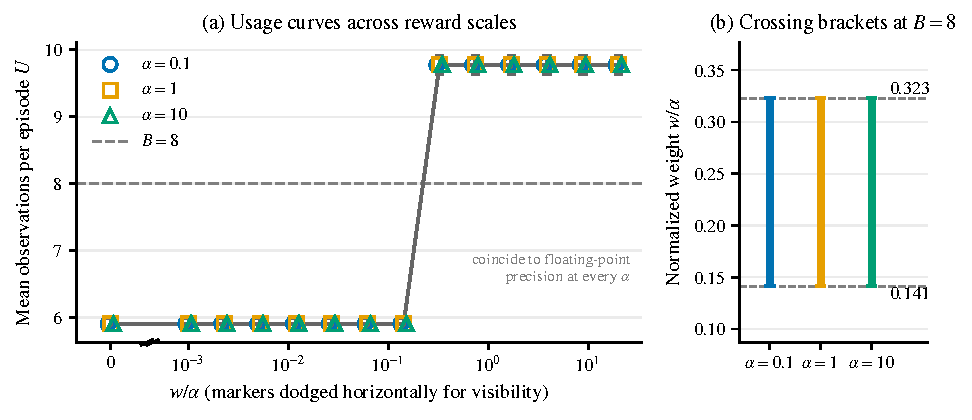
\includegraphics[width=\textwidth]{figures/price_scale_invariance.pdf}
\caption{Reward-scale transfer on Diagnosis. In (a), separately evaluated usage curves shift when rewards and sensing costs are multiplied by $\alpha\in\{0.1,1,10\}$. In (b), plotting against $w/\alpha$ collapses them exactly, including the $B{=}8$ grid bracket $(0.141,0.323]$. Points and error bars are means $\pm1$ seed-level SE over five seeds and $100$ episodes per seed, with shared per-episode streams. Lines guide the eye. Bands and open--closed endpoints mark grid brackets, not uncertainty intervals or policies attaining the target. The crossing between sampled points remains unresolved.}
\label{fig:collapse}
\Description{Two panels use the same usage scale. On the left, three separately evaluated Diagnosis curves shift to larger information weights as the reward and sensing-cost multiplier increases from 0.1 to 1 to 10. Their open circle, square, and triangle markers lie near usage 6 below the transition and near 10 above it. Colored bands mark three separated grid brackets where the curves cross the dashed target at 8. On the right, the same rows are plotted against weight divided by the multiplier. All three marker types overlap at their actual coordinates, and one gray band marks the common grid bracket from 0.141 to 0.323.}
\end{figure}

\subsection{Online Re-adaptation after a Reward Rescale}
\label{sec:dual_multiseed}

We compare the projected decaying-step controller with its reset-on-shift extension on Diagnosis at target $B{=}8$. Both use $\eta_0{=}0.05$, decay $\delta{=}0.02$, and a tenfold reward-and-cost rescale at episode $200$ of a $400$-episode run. Ten shared controller seeds support a paired comparison. The extension watches a $20$-episode usage window. Once the step has decayed below half its initial value, a deviation exceeding both three window standard errors and $0.5$ observations restarts its decay clock. Appendix~\ref{app:dual_details} specifies the detector and steady-state summaries.

Recovery occurs when a rolling mean computed only from post-rescale episodes stays within $\pm1$ of $B$ for $20$ consecutive episodes. The comparison uses the restricted time $\min(T,180)$ for every seed, where $180$ is the last post-rescale index at which that hold can be checked. A seed that never completes it receives $180$. Decay-only averages $157.3$ episodes and reset-on-shift $51.2$, a descriptive ratio of $3.07$. The paired difference is $106.1$ episodes with a Student-$t$ $95\%$ interval $[96.8,115.4]$. All ten paired differences favor resetting. Reset-on-shift recovers on $10/10$ seeds and decay-only on $9/10$, so the latter's unrestricted recovery distribution is right-censored. The conditional mean among its nine recovered seeds is not the comparison estimand.

These measurements come from the corrected per-episode-seeded runner. The earlier runner left the rescaled environment unseeded and reported a ratio of $2.65$ with all decay-only seeds recovering. The correction preserves the qualitative advantage while revealing slower and incomplete recovery for decay-only. Figure~\ref{fig:dualmultiseed} plots the trajectories. The mid-run rescale is nonstationary, and the reset variant restarts its step schedule, so neither experiment is covered by Proposition~\ref{prop:pi5}'s stationary convergence guarantee. This is empirical re-adaptation evidence on one shift scenario.

\begin{figure}[tbp]
\centering
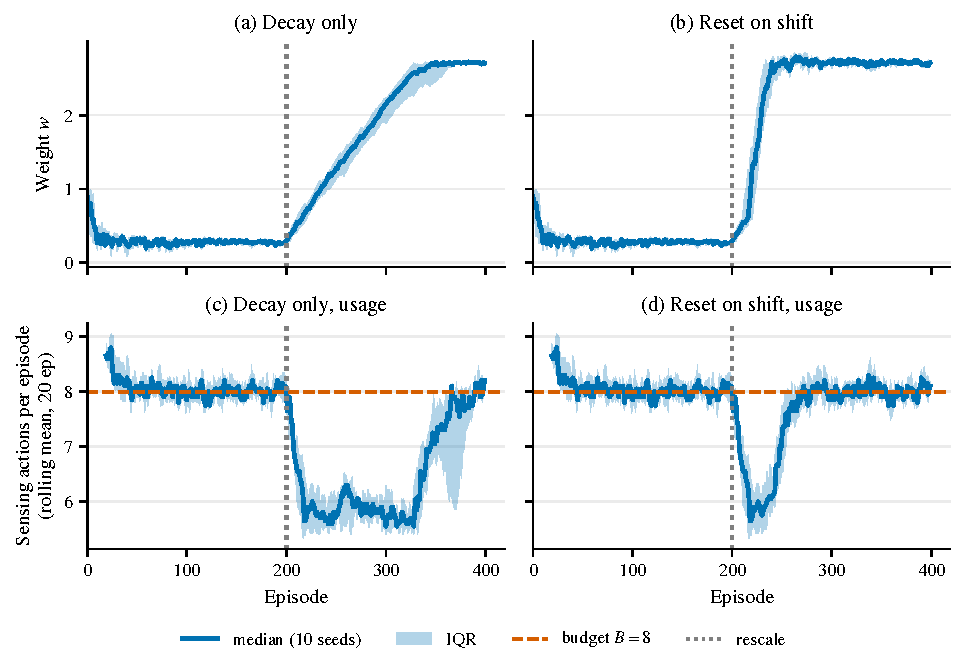
\includegraphics[width=\textwidth]{figures/price_dual_multiseed.pdf}
\caption{Online control on Diagnosis through a tenfold reward-and-cost rescale at episode $200$. Columns compare decay-only and reset-on-shift. Top panels show weight, as median and interquartile range over ten seeds. Bottom panels show rolling usage with window $20$ and target $B{=}8$. Recovery uses post-shift-only windows and a $20$-episode hold within $\pm1$ of the target. Restricted recovery time $\min(T,180)$ averages $157.3$ versus $51.2$ episodes, with paired difference $106.1$ and Student-$t$ $95\%$ interval $[96.8,115.4]$. This nonstationary experiment is outside Proposition~\ref{prop:pi5}.}
\label{fig:dualmultiseed}
\Description{A two-by-two grid of time series over 400 episodes, with one column per controller variant. Top row. The median weight trajectory with a shaded interquartile band drops from about 1 to about 0.3, holds flat until the dotted vertical line at episode 200, then climbs to about 2.7. The left variant climbs gradually over roughly 150 episodes while the right variant jumps up within about 50 episodes. Bottom row: rolling median usage hovers on the dashed budget line at 8, dips to between about 5 and 6 after the shift, and returns to the budget line, slowly on the left and quickly on the right.}
\end{figure}

\subsection{Cost-Denominated Budgets}
\label{sec:cost_budget}

The count-usage curves of Section~\ref{sec:collapse} treat every observation as one unit regardless of price. Section~\ref{sec:budget_solve} noted that usage can instead be denominated in cumulative sensing cost, and that the two denominations agree only when every observation action costs the same. This subsection demonstrates end to end that the denomination matters. A budget stated in test count and a budget stated in sensing cost are not interchangeable, because the agent's mix of cheap and expensive tests can change with $w$. We introduce a Diagnosis variant with heterogeneous per-test costs. Its two test types are priced differently, the cheaper test at $0.5$ and the more expensive test at $2.5$ (the cost vector $[0.5, 2.5]$ in the implementation), while both tests keep the base environment's accuracy. On this variant we estimate both the count-usage curve $U_{\mathrm{count}}(w)$ and the cost-usage curve $U_{\mathrm{cost}}(w)$ on the same agent family.

The mechanism is a shift in the agent's test mix. Recall from Section~\ref{sec:experiments} that each Diagnosis test reports, noisily, which side of its own fixed split of the hidden conditions the true condition lies on, and that the two tests use different splits. The two tests are equally accurate, but because their splits differ, how much each reveals depends on how the current belief is spread across its split. At a given belief one test can therefore reveal more than the other. What the swept curves show is a step. The mean cost paid per test, $U_{\mathrm{cost}}(w)/U_{\mathrm{count}}(w)$, holds at $1.26$ from $w{=}0$ through $w{=}10$ and rises to $1.37$ and then $1.41$ only at the two largest weights, the same two weights at which the number of tests also jumps (Figure~\ref{fig:costbudget}), a $12.0\%$ spread relative to the grid-mean cost per test. Our reading of the step is an interpretation rather than a measurement. While information gain is weighted lightly, the price holds the agent to its low-weight test mix, and once $w$ is large enough to buy extra tests, test choice is driven more by what a test reveals at the current belief than by its price, which on this variant means using the expensive test more often. The direction is measured on the swept curves rather than implied by the cost vector, which by itself says nothing about which test reveals more. A count budget cannot see that shift, while a cost budget prices it. This confirms directly that the two denominations are not interchangeable.

Whether the two denominations also select different weights at a given budget is a separate question, and answering it requires a rule for pairing a count budget with a cost budget. A cost budget here is not a count budget converted through a cost per test. Instead each curve is measured on its own scale, and the two budgets of a pair are set at the same fractional height inside each curve's own usage range. The usage range of a curve is the span from the smallest to the largest mean usage on the tested grid. A margin is held back at both ends of that span before budgets are placed, so that each budget has a crossing bracket on the grid. We call two budgets paired in this way comparable operating points. Since the two denominations are not interchangeable, one might expect them to select different brackets at such a pair. At the two comparable operating points we solve for, however, they happen to land in the same crossing bracket at this grid's resolution. A count budget $B{=}8.86$ has crossing bracket $(10, 31.6]$, and a cost budget $B_{\mathrm{cost}}{=}11.50$ (the comparable operating point on the cost curve, a budget on total sensing cost rather than on test count) also has crossing bracket $(10, 31.6]$ (Figure~\ref{fig:costbudget}). The same coincidence holds at the higher pair of budgets we test ($B{=}13.71$ count, $B_{\mathrm{cost}}{=}19.20$ cost, both with crossing bracket $(31.6, 100]$).

The coincidence has a simple explanation. The cost curve is the count curve multiplied by the mean cost per test. If that multiplier were the same at every weight, the pairing rule would make the two crossings coincide exactly, because a budget at a given fractional height of the count curve and the budget at the same fractional height of the cost curve would then be one and the same budget written in two units. The two curves would then cross them at the same weight. Only the variation of the multiplier across the grid can pull the two crossings apart, by shifting where along the weight axis the cost curve crosses its budget. That multiplier moves by at most the $12\%$ spread just reported, while adjacent positive grid weights are log-spaced a factor of $\sqrt{10} \approx 3.2$ apart. A bracket changes only if that shift carries the crossing past one of those grid weights. A rescaling that small need not carry a crossing into a neighboring grid cell, and at these two pairs it does not. The two denominations are therefore not guaranteed to disagree at every tested budget pair. They land in different brackets only when the variation in the cost per test is large enough, relative to the grid's resolution, to move a crossing past a grid weight.

\begin{figure}[tbp]
\centering
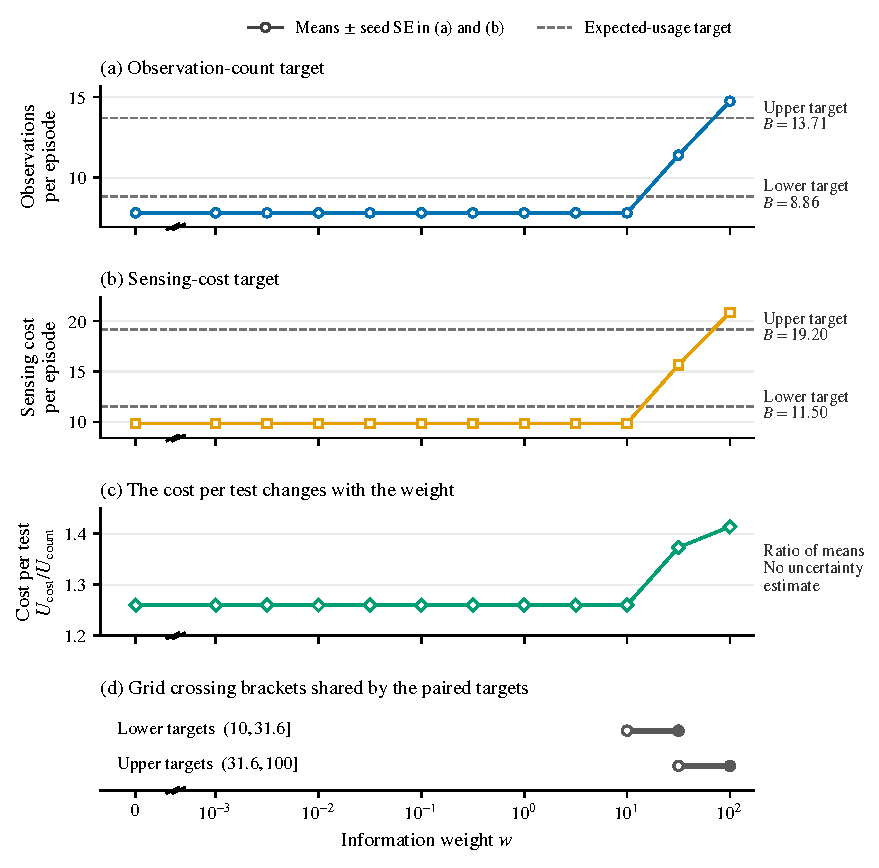
\includegraphics[width=\textwidth]{figures/price_cost_budget.pdf}
\caption{Observation-count and sensing-cost targets on heterogeneous-cost Diagnosis. Panels (a) and (b) separate the two usage units, showing means $\pm 1$ seed-level SE and the tested targets as dashed lines. The lower count/cost targets are $8.86/11.50$, and the upper targets are $13.71/19.20$. Panel (c) shows the ratio of mean sensing cost to mean observation count, which rises as the test mix changes. No uncertainty estimate is shown for this ratio. Panel (d) displays the paired targets' shared crossing brackets, $(10,31.6]$ and $(31.6,100]$. These intervals measure grid resolution, not statistical uncertainty. Lines joining sampled means guide the eye.}
\label{fig:costbudget}
\Description{Four vertically aligned panels share information-weight coordinates. The first shows a blue observation-count curve with seed-level error bars, the second an orange sensing-cost curve with seed-level error bars, and the third a green ratio-of-means curve without an uncertainty estimate. The last panel shows two gray open-left, closed-right grid-bracket bars. Target labels are outside the data panels, the legend sits above them, and there is no background shading.}
\end{figure}

\subsection{RockSample and Structural Inspection as Interleaved Settings}
\label{sec:interleaved_budget}

We now estimate usage curves and shadow prices in settings where sensing and acting alternate within an episode, the interleaved observe-act settings of Section~\ref{sec:rocksample} and Section~\ref{sec:inspection}. The extension is needed because Proposition~\ref{prop:factored}'s factored-observation class admits navigation actions between observations, so that sensing and acting can alternate, whereas the observe-then-commit environments above separate observation from commitment by construction and so cannot exercise that case. We use the interleaved tree-search agents that those two sections specify, counting check/test actions as sensing usage. The three instances are RockSample[5,3], RockSample[7,4], and Inspection-$N{=}16$. All three share one set of five seeds, and every episode count below is per seed at each grid weight. RockSample[5,3] uses a $10$-point weight grid with $5$ seeds $\times$ $50$ episodes, and its usage range (Section~\ref{sec:cost_budget}) is $[3.00, 8.83]$. RockSample[7,4] uses an $8$-point grid with $30$ episodes and spans $[2.00, 14.54]$. Inspection-$N{=}16$ uses a $10$-point grid with $50$ episodes and spans $[22.38, 58.56]$. Budgets are placed inside each usage range by the rule of Section~\ref{sec:cost_budget}, at evenly spaced positions, with a narrower margin held back at each end than that section used. Inspection appears at $N{=}16$, the larger of the two instances evaluated in Section~\ref{sec:inspection}, while the staircases of Section~\ref{sec:stairs} use the smaller $N{=}8$ instance. The two subsections together therefore cover both sizes. Figure~\ref{fig:interleaved} reports grid estimates of the shadow prices for each instance. Four budgets are evaluated per environment, each reported with a crossing bracket and the usage SE at its plotted grid weight.

The usage curves $U(w)$ from which these staircases are read off are nondecreasing between every pair of consecutive sampled grid points on RockSample[7,4] and Inspection-$N{=}16$. That is cleaner than the count-usage curves of Bandit and Tileworld, which the discussion after Proposition~\ref{prop:pi2} noted are only roughly monotone and whose shadow-price staircases follow in Section~\ref{sec:stairs}. RockSample[5,3] is the exception to this clean monotonicity. Its instrumental floor, the usage the agent spends at $w{=}0$ because reward alone already motivates that much sensing, is $U(0){=}3.70 \pm 0.11$ (SE), and usage dips from there down to $3.00 \pm 0.00$ at $w{=}0.316$ before rising, a gap of roughly six SEs. This is the same kind of non-monotone dip the observe-then-commit environments show, so the interleaved class does not uniformly enjoy the cleaner monotonicity of the other two instances.

On the sampled RockSample[7,4] and Inspection-$N{=}16$ grids, the smallest measured usage occurs at $w=0$, so no tested weight meets a lower target. The usages at zero weight are $U(0)=3.70$ on RockSample[5,3], $2.00$ on RockSample[7,4], and $22.38$ on Inspection-$N{=}16$. These measurements identify lower limits within the sampled grids, not bounds for every untested weight. They show why attainable usage must be checked in interleaved settings as well as in the observe-then-commit class. RockSample[5,3] is again the exception, because there a positive weight buys less sensing than $w{=}0$ does, so budgets between $3.00$ and $3.70$ are achievable even though they lie below $U(0)$. The lowest RockSample[5,3] budget in Figure~\ref{fig:interleaved} lies in this band. The figure draws it as slack because the grid weight whose usage comes nearest to that budget is $w{=}0$ itself, which sits below the budget's crossing bracket, not because the budget is unachievable.

\begin{figure}[tbp]
\centering
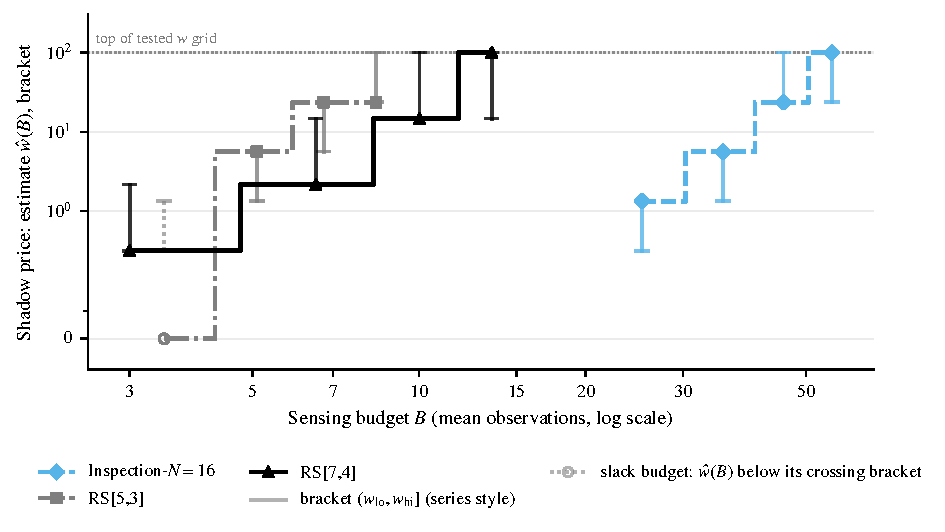
\includegraphics[width=\textwidth]{figures/price_staircase_interleaved.pdf}
\caption{Grid estimates of the shadow price on three interleaved (non-observe-then-commit) settings, RockSample[5,3], RockSample[7,4], and Inspection-$N{=}16$, with crossing brackets marked as vertical bars, capped where they reach the dotted rule marking the top of the tested $w$ grid, and an open-circle marker where a budget is slack (the grid weight whose usage comes nearest to the budget sits strictly below the bracket's lower edge, here $w{=}0$ on the lowest RockSample[5,3] budget). Every marker plots the nearest-point solution $\hat{w}(B)$, which can sit on a bracket's lower edge. The budget axis is logarithmic and the weight axis uses a symmetric-log scale, linear near zero. The underlying usage curves $U(w)$ are monotone at every sampled grid point on RockSample[7,4] and Inspection-$N{=}16$, while RockSample[5,3] dips once near $w{=}0.316$ before rising (see text).}
\label{fig:interleaved}
\Description{A single step plot of shadow price against sensing budget, with a logarithmic budget axis and a symmetric-log weight axis, linear near zero, running from zero to 100 and a dotted rule marking the top of the tested weight grid. Three staircases in gray, black, and light blue. All three staircases rise from left to right without any downward step. The gray RockSample[5,3] staircase starts at an open-circle slack marker at a price of 0 and a budget of about 3.5 and climbs to a price of about 24 by a budget of about 6.7, the black RockSample[7,4] staircase climbs from a price of about 0.3 at a budget of about 3 to a price of 100 at a budget of about 13.5, and the light blue Inspection staircase sits farthest right, climbing from a price of about 1.3 at a budget of about 25 to a price of 100 at a budget of about 56. Vertical bars in each series' color mark the crossing bracket at each step point, capped at both ends, and the bars whose upper edge is the top of the tested weight grid end exactly on the dotted rule at 100.}
\end{figure}

\subsection{Shadow-Price Staircases across Five Domains}
\label{sec:stairs}

The observe-then-commit domains and the smaller Inspection instance now receive the same treatment as the interleaved instances. Figure~\ref{fig:stairs} reports grid estimates of $w^*(B)$ over identifiable budgets inside $[U_{\min}, U_{\max}]$ for Tiger, Diagnosis, Bandit, Tileworld-$6{\times}6$, and Inspection-$N{=}8$, where $U_{\min}$ and $U_{\max}$ are the endpoints of each curve's usage range (Section~\ref{sec:cost_budget}). An identifiable budget is one placed strictly inside that range by the rule of that section, evenly spaced with the same margin held back at each end as in Section~\ref{sec:interleaved_budget}, so that the grid brackets it. The monotonicity at issue is that of the underlying usage curve $U(w)$ from which each staircase is read off, taken between consecutive sampled grid weights. On Tiger, Diagnosis, and Inspection that curve is nondecreasing between every pair of consecutive grid weights. On Bandit and Tileworld it is not, showing local non-monotonicity from discrete policy switches, the first of the two obstacles noted after Proposition~\ref{prop:pi2}. We report crossing brackets and usage standard errors for every domain (Definition~\ref{def:pi3}). The standard error attached to a bracket is that of usage at a fixed weight, and the bracket's width is set by the grid, so neither says how often a different sample of seeds would select a different bracket. We measured that directly. Resampling the five seeds with replacement $2000$ times and re-solving each of the $25$ budgets of Figure~\ref{fig:stairs} on the resampled curve (\texttt{run\_\allowbreak bracket\_\allowbreak stability.py}, \texttt{results\_\allowbreak price\_\allowbreak bracket\_\allowbreak stability.csv}, with the count of every bracket outcome in \texttt{results\_\allowbreak price\_\allowbreak bracket\_\allowbreak stability\_\allowbreak counts.csv}), the reported bracket is recovered in every resample at $19$ budgets and in at least $99$ percent of resamples at $21$. The lowest agreement is $0.789$, at Inspection's lowest budget. In every disagreeing resample but one, the alternative is a neighbouring step of the staircase or, at Tiger's lowest and highest budgets, which lie about one standard error of usage from the two ends of its usage range, no bracket at all. On Bandit and Tileworld a budget can be crossed more than once, and the reported bracket estimates the last crossing by the convention that definition adopts, so it names one threshold at grid resolution rather than displaying the reversals. Bandit's budget $B{=}5.87$ is the one tested case. Usage first reaches it at $w{=}0.139$ ($6.19$ observations), falls back to $5.11$ at $w{=}0.72$, and reaches it for the last time inside the reported bracket $(1.64, 3.73]$ (\texttt{results\_\allowbreak price\_\allowbreak shadow\_\allowbreak curves.csv}), which does not show the earlier crossing. Tiger's price is weakly identified, consistent with Table~\ref{tab:collapse-breadth}, in the sense that the budget pins the price down only loosely. Instrumental listening already saturates most of the usage range at $w{=}0$, so the curve is flat at its floor across the low-weight range and rises in a single step at high weight. Every tested budget lands in that one step's bracket.

\begin{figure}[tbp]
\centering
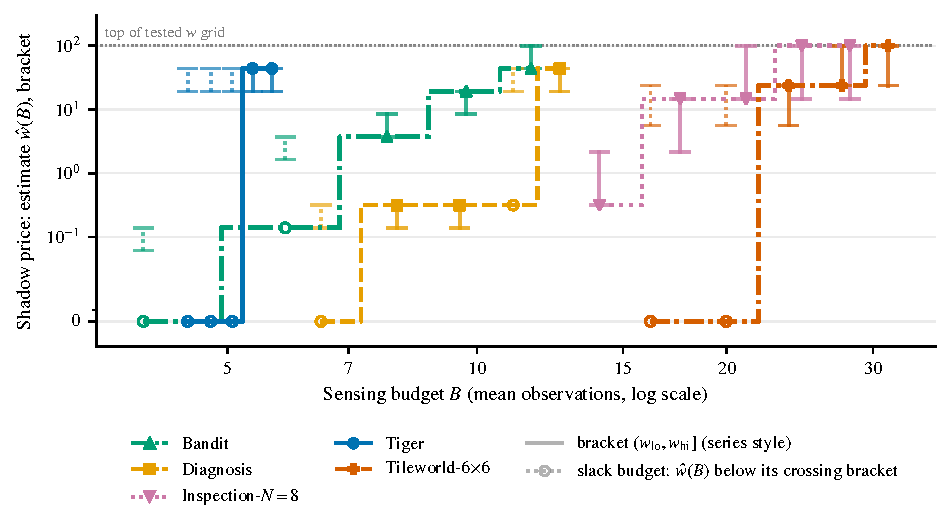
\includegraphics[width=\textwidth]{figures/price_shadow_curves.pdf}
\caption{Operational shadow-price staircases $w^*(B)$ across five observe-then-commit and inspection domains (Tiger, Bandit, Diagnosis, Inspection-$N{=}8$, Tileworld-$6{\times}6$), each in its own color, with a logarithmic budget axis and a symmetric-log weight axis that is linear near zero. Each staircase steps up as the sensing budget $B$ rises, and the vertical bar at each step marks that budget's crossing bracket $(w_{\mathrm{lo}}, w_{\mathrm{hi}}]$ (Definition~\ref{def:pi3}), capped where the bracket's upper edge coincides with the top of the tested $w$ grid (dotted horizontal rule at $100$). An open circle with a dotted bar marks a slack budget, one for which the grid weight whose usage comes nearest to the budget lies strictly below the lower edge of the crossing bracket ($w{=}0$ at seven of the nine marked budgets, $w{=}0.316$ at Diagnosis $B{=}11.06$, and $w{=}0.139$ at Bandit $B{=}5.87$, the twice-crossed budget discussed in the text), so the nearest-point solution returns a weight below the bracket while the dotted bar still marks the crossing. Every marker plots that nearest-point solution $\hat{w}(B)$, which can also sit on a bracket's lower edge. The usage curves behind Tiger, Diagnosis, and Inspection never step downward between consecutive sampled weights, while Bandit and Tileworld show local non-monotonicity from discrete policy switches, so their brackets mark the last crossing of each budget by the convention of Definition~\ref{def:pi3}.}
\label{fig:stairs}
\Description{A single plot of shadow price against a logarithmic sensing-budget axis, with a symmetric-log vertical axis that is linear near zero, with five colored staircase curves and vertical bracket bars drawn in each series' own color, capped at both ends and ending exactly on the dotted rule at 100 where the bracket's upper edge is the top of the tested weight grid, with open markers and dotted bars at slack budgets. The blue Tiger staircase rises almost vertically near a budget of about 5.2. The green Bandit and orange Diagnosis staircases climb between budgets of roughly 4 and 13. The pink Inspection and vermillion Tileworld staircases climb between roughly 14 and 31. Tiger, Bandit, and Diagnosis step upward from zero to a top price of about 44, while Inspection and Tileworld reach 100, some with locally uneven step placement.}
\end{figure}

\subsection{Unconstrained Reward Reference}
\label{sec:sarsop}

To determine whether $w{=}1$ is reward-competitive at its natural operating point, we compare EFE with SARSOP \citep{kurniawati2008} on Tiger, Diagnosis, and Bandit. The original APPL solver is built from source, each environment is exported through a common model path, and the solve uses precision $10^{-3}$ at $\gamma{=}0.999$. The returned alpha-vector policy is evaluated in the same simulator as EFE at five seeds and $500$ episodes per seed (Table~\ref{tab:sarsop}). SARSOP is a near-optimal reference, not a certified exact solution to the reported Monte Carlo comparison. Build and export details appear in Appendix~\ref{app:sarsop_build}.

\begin{table}[t]
\centering
\caption{SARSOP and EFE ($w{=}1$) on the three core environments, five seeds and $500$ episodes per seed, $\gamma{=}0.999$. Values are means $\pm$ seed-level SE. Usage counts observations. Fixed-margin TOST and its retrospective/prospective scope are described in the text.}
\label{tab:sarsop}
%% Numbers in this table are produced by experiments/run_sarsop_baseline.py
\tablefontsize
\begin{tabular}{lcccc}
\toprule
Environment & SARSOP reward & EFE reward & SARSOP usage & EFE usage \\
\midrule
Tiger & $5.061 \pm 0.158$ & $5.061 \pm 0.158$ & $4.323 \pm 0.045$ & $4.323 \pm 0.045$ \\
Diagnosis & $-1.452 \pm 0.336$ & $-1.217 \pm 0.184$ & $9.68 \pm 0.12$ & $9.73 \pm 0.13$ \\
Bandit & $6.280 \pm 0.134$ & $6.261 \pm 0.112$ & $5.16 \pm 0.09$ & $5.09 \pm 0.07$ \\
\bottomrule
\end{tabular}
\end{table}

Tiger's policies take identical actions on every evaluated episode. Diagnosis and Bandit show small reward differences, but non-significance alone would not establish equivalence. We therefore use two one-sided tests (TOST) \citep{schuirmann1987} with a reward margin equal to one observation's cost, $\pm1.0$ on Tiger and Diagnosis and $\pm0.5$ on Bandit. These operational margins were chosen after an earlier canonical-seed comparison had been inspected, so the five-seed TOST is retrospective. The additional fifteen seeds in the $n{=}20$ robustness study were fixed after the margin and before that study ran.

The primary TOST uses unpaired Welch tests on per-seed means. All three environments reject both one-sided nulls, including after Holm correction across environments, with $p_{\mathrm{TOST}}=0.0010$, $0.0458$, and $0.0130$ for Tiger, Diagnosis, and Bandit. Their $90\%$ intervals lie inside the specified margins. The $n{=}20$ study retains equivalence, with respective $p$-values $4.5{\times}10^{-10}$, $6.8{\times}10^{-7}$, and $6.0{\times}10^{-11}$. The nominal seed lists are shared, but differing policies consume random draws differently. A paired five-seed sensitivity analysis confirms that covariance is positive here and the unpaired analysis is conservative. Tiger's paired differences are identically zero. Diagnosis and Bandit give paired $p_{\mathrm{TOST}}$ of $0.016$ and $3.6{\times}10^{-5}$. Appendix~\ref{app:sarsop_details} gives intervals, mechanics, and archive filenames. The conclusion is equivalence within these fixed margins on these three environments, rather than universal near-optimality of $w{=}1$.

\subsection{A Usage-Constrained Reference}
\label{sec:cpomdp}

A literal usage penalty supplies a different reference from an information bonus. We replace observation reward $-\mathrm{cost}_j$ by $-(\mathrm{cost}_j+\lambda)$ and solve with SARSOP over a $12$-point penalty grid in $[0,100]$. This estimates policies maximizing $\mathbb E[R]-\lambda\mathbb E[U]$ over the POMDP policy space, with $\gamma{=}0.999$ and five seeds of $300$ episodes per penalty. The penalty is the Lagrangian price of the usage cap in Equation~\ref{eq:budgeted}. The information weight $w$ is not that multiplier.

At budget $B$, the reference is the feasible envelope of the sampled policy points, obtained by maximizing their mixture reward subject to mixture usage at most $B$. A solution uses at most two sampled policies. Policies below the target remain eligible, and the reference is flat at the largest sampled reward once the cap is slack. This is a linear program over measured points, not equal-usage interpolation. The solver is approximate, the penalty grid is finite, and reward and usage are Monte Carlo estimates. Consequently the envelope is neither a certified population bound nor the full constrained frontier. We do not assume that finite-state strong-duality results \citep{altman1999} automatically extend to the continuous belief MDP. Appendix~\ref{app:cpomdp_details} discusses these limitations and the diagnostic interpolation retained in the CSV.

\begin{table}[h]
\centering
\caption{Estimated cap-constrained reference at EFE usage $B_{\mathrm{EFE}}$. $R_{\mathrm{ref}}$ maximizes reward over mixtures of sampled SARSOP-Lagrangian policies with usage at most that budget. Gap is $R_{\mathrm{ref}}-R_{\mathrm{EFE}}$, not a certified optimality gap. On each environment the best sampled reference is already feasible, so the cap does not bind. Values use five seeds and $300$ episodes per seed. The actually evaluated usage-matched Planning+IG grid weights produce the same rewards as EFE in this run.}
\label{tab:cpomdp}
%% Numbers in this table are produced by experiments/run_cpomdp_baseline.py
\tablefontsize
\begin{tabular}{lccccc}
\toprule
Environment & $B_{\mathrm{EFE}}$ & $R_{\mathrm{ref}}$ & $R_{\mathrm{EFE}}$ & Gap & Gap \% \\
\midrule
Tiger & $4.32$ & $5.016$ & $5.016$ & $0.000$ & $0.00\%$ \\
Diagnosis & $9.82$ & $-1.265$ & $-1.224$ & $-0.041$ & $-3.27\%$ \\
Bandit & $5.10$ & $6.314$ & $6.320$ & $-0.005$ & $-0.08\%$ \\
\bottomrule
\end{tabular}
\end{table}

Table~\ref{tab:cpomdp} evaluates the reference at EFE's endogenous usage $B_{\mathrm{EFE}}$. The highest-reward sampled reference policy is already feasible on each environment, so the cap does not bind. Its estimated gap from EFE is zero on Tiger, $-0.041$ on Diagnosis, and $-0.005$ on Bandit, small relative to the estimates' standard errors. Negative estimated gaps can arise from sampling or approximation error and do not establish reward above the population optimum. The usage-matched Planning+IG grid weights actually run, $0.00$, $0.45$, and $1.07$, give rewards bit-identical to EFE here. This is an empirical plateau result rather than an extension of the equivalence theorem from $w{=}1$ to arbitrary weights. The reference remains limited to these small environments, with no corresponding optimality-gap estimate for the larger RockSample and Inspection instances.

\subsection{Calibration-Derived Targets on Held-Out Seeds}
\label{sec:budget_frontier}

The preceding comparison uses whatever sensing the weight-one policy happens to buy. We now test targets independent of that weight-one usage, chosen by a predeclared rule from each calibration curve. These targets stand in for application requirements but are not themselves application-specified. The study separates whether the procedure meets expected usage from whether doing so maximizes reward under a cap. Its original design was recorded in the producer's docstring before results were inspected (\texttt{experiments/\allowbreak run\_\allowbreak budget\_\allowbreak frontier.py}).

Each core environment is calibrated on the canonical five seeds, $100$ episodes per seed, using the $16$-point weight grid and horizons of Section~\ref{sec:stairs}. We select budgets at $0.25$, $0.5$, and $0.75$ of the measured range $[U_{\min},U_{\max}]$, at the midpoint of its largest jump, and at half of $U_{\min}$. The last is deliberately unattainable and must be declared so. Definition~\ref{def:pi3} supplies the crossing bracket and endpoint-mixture probability $q$. All selection uses calibration data alone, and evaluation uses held-out seeds $\{7,8,9,10,11\}$ with $100$ episodes each. Tiger's gap budget duplicates its middle-range budget. Bandit's curve is nonmonotone, so the stipulated last-crossing convention determines its bracket.

The original within-family comparator is the highest-reward single grid member whose calibration usage is at most $B$. Two additional LP comparators were introduced after inspecting the first results, and that amendment is disclosed in the producer. One maximizes calibration reward over mixtures with usage equal to $B$, and one does so with usage at most $B$. Each uses at most two calibration-grid weights and is evaluated on held-out seeds. Their scope is the sampled grid. Selecting calibration usage below a cap does not guarantee that the population or held-out usage meets it.

Table~\ref{tab:budget_frontier_main} gives the principal held-out results. All three below-range targets are declared unattainable. At all twelve attainable targets, the selected endpoint mixture meets usage to within $0.13$ observations. Errors are within one held-out SE except Bandit's gap target, where an error of $0.09$ is about $1.3$ SE. The evaluated bracket endpoints and best feasible single member miss the targets by more. Endpoints miss by $0.3$--$1.1$ observations on Tiger and $0.2$--$3.6$ elsewhere. The selected feasible single member leaves $0.2$--$4.7$ observations unspent on held-out data. Its usage is below the target in all twelve rows, an observed result in addition to the calibration selection fact. Conversely, the endpoint mixture's held-out mean exceeds $B$ on three rows, by at most $0.13$. An expected-use target provides neither a hard per-episode cap nor finite-sample cap feasibility.

\begin{table}[t]
\centering
\caption{Endpoint-mixture calibration on held-out seeds, $100$ episodes per seed over five seeds. $B$ is the calibration-derived expected-use target. $U$ and $R$ are held-out mixture usage and reward. All $\pm$ values are seed-level SE. The paired gap is mixture reward minus the same-stream cap-reference envelope, with seed-level SE. Its support and weights are fitted on those same seed means and held fixed for the SE, so intervals derived from this column are nominal pointwise plug-in summaries, as qualified in the text. Tiger's gap row duplicates its middle target. All three below-range targets are declared unattainable. Complete within-family and reference comparisons appear in Table~\ref{tab:budget_frontier}.}
\label{tab:budget_frontier_main}
%% All numerical cells copied from tables/budget_frontier.tex, produced by
%% experiments/run_budget_frontier.py and run_frontier_reference_heldout.py.
\tablefontsize
\setlength{\tabcolsep}{4pt}
\begin{tabular}{@{}llcccc@{}}
\toprule
Environment & Target & $B$ & $U$ & $R$ & Paired gap \\
\midrule
Tiger & 0.25 & $4.72$ & $4.64 \pm 0.10$ & $5.36 \pm 0.10$ & $-0.33 \pm 0.04$ \\
Tiger & 0.50 & $5.07$ & $5.04 \pm 0.14$ & $4.96 \pm 0.14$ & $-0.72 \pm 0.06$ \\
Tiger & 0.75 & $5.42$ & $5.35 \pm 0.14$ & $4.65 \pm 0.14$ & $-1.03 \pm 0.06$ \\
Tiger & gap & $5.07$ & $5.04 \pm 0.14$ & $4.96 \pm 0.14$ & $-0.72 \pm 0.06$ \\
\midrule
Diagnosis & 0.25 & $7.72$ & $7.70 \pm 0.25$ & $-2.14 \pm 0.48$ & $-0.03 \pm 0.28$ \\
Diagnosis & 0.50 & $9.53$ & $9.47 \pm 0.20$ & $-2.11 \pm 0.67$ & $-0.76 \pm 0.15$ \\
Diagnosis & 0.75 & $11.35$ & $11.47 \pm 0.37$ & $-2.31 \pm 0.45$ & $-1.10 \pm 0.22$ \\
Diagnosis & gap & $7.84$ & $7.86 \pm 0.25$ & $-2.06 \pm 0.47$ & $0.00 \pm 0.22$ \\
\midrule
Bandit & 0.25 & $5.51$ & $5.62 \pm 0.21$ & $6.06 \pm 0.26$ & $-0.21 \pm 0.12$ \\
Bandit & 0.50 & $7.79$ & $7.67 \pm 0.37$ & $5.70 \pm 0.25$ & $-0.57 \pm 0.09$ \\
Bandit & 0.75 & $10.07$ & $9.95 \pm 0.36$ & $4.95 \pm 0.22$ & $-1.32 \pm 0.08$ \\
Bandit & gap & $4.71$ & $4.62 \pm 0.07$ & $5.62 \pm 0.21$ & $-0.59 \pm 0.20$ \\
\bottomrule
\end{tabular}
\end{table}

Meeting a target can buy useful information or impose an avoidable reward cost. On Diagnosis at $B{=}7.72$, $9.53$, and its gap target $7.84$, the mixture earns $-2.14$, $-2.11$, and $-2.06$ against the feasible member's $-2.86$. On Tiger, reward-only planning uses $4.32$ observations and earns $5.68$ on this held-out stream. Spending more to meet the three increasing targets reduces reward to $5.36$, $4.96$, and $4.65$. Bandit likewise loses reward at its two larger interior targets. The endpoint procedure also need not select the best mixture meeting a target. At Bandit's gap budget, the calibration LP mixes $w{=}0$ and $w{=}0.72$ and earns $5.94\pm0.19$ on held-out seeds, against the endpoint mixture's $5.62\pm0.21$. Its usage error is larger, $0.18$ rather than $0.09$. The chosen endpoint mixture therefore cannot stand for every mixture in the family, and its deficit at this budget cannot be attributed to planning depth alone.

A valid constrained-reward comparison must also control the evaluation stream. The original reference points were evaluated on canonical seeds with once-per-seed seeding, whereas the family uses held-out per-episode seeds. Their direct reward comparisons, retained in Appendix~\ref{app:frontier_details}, are descriptive cross-stream comparisons. The difference matters on Tiger. Its unpenalized reference earns $5.02$ on the canonical stream but $5.68$ on the held-out stream, removing the mixture's apparent excess over the reference at the smallest budget.

We therefore added a same-stream comparison after inspecting the original results. Every saved reference policy was first checked against its committed canonical estimate to $10^{-9}$, then re-evaluated on the held-out seeds with the family's per-episode seeding, and the feasible envelope was recomputed. The final column of Table~\ref{tab:budget_frontier_main} pairs each seed's mixture reward with its reference reward on the same episode seeds. Reference support and mixture weights are fitted on those same held-out seed means and held fixed for the SE. The resulting Student-$t$ intervals are nominal pointwise plug-in summaries. They omit support reselection, uncertainty in mixture weights and cap feasibility, and multiplicity across budgets. They do not establish coverage for the population constrained frontier.

Under that fitted comparison, negative $95\%$ intervals exclude zero at nine of twelve attainable budgets, or eight of eleven distinct budgets after the Tiger duplicate is removed. The largest measured shortfall is $1.32$ on Bandit, about one fifth of its reference reward. Three intervals include zero, at Diagnosis's smallest and gap targets and Bandit's smallest target. Re-evaluation removes the stream mismatch but leaves selection bias from maximizing over noisy reference points.

Tiger requires an additional rare-event qualification. Neither the family nor any policy in the fitted reference support makes a wrong commit in the $500$ held-out episodes. Its paired gaps therefore measure only extra listening. A wrong commit costs $110$ relative to a correct one, and the canonical reference error rate is $0.6\%$, equivalent to about $0.66$ expected reward. If the reference retained that rate while the family never erred, the smallest-budget shortfall would reverse and the middle-budget shortfall would nearly vanish. Only the largest Tiger shortfall is robust to that sensitivity calculation. The nominal intervals do not capture this rare-event uncertainty.

This study supports expected-usage calibration within the tested family, including gap targets, while quantifying its limits as a reward optimizer. If the engineering requirement is to spend a specified expected sensing amount for coverage or verification that reward does not represent, the endpoint mixture directly addresses it. If the requirement is only an upper limit and reward is the objective, the feasible mixture or constrained reference is the relevant comparator. The complete three-panel table, selection details, historical reference correction, and paired archives are retained in Appendix~\ref{app:frontier_details}.

\subsection{Reward-Irrelevant Sensing}
\label{sec:distractor}

An expected sensing target controls the amount of sensing, but does not ensure that it concerns the task. We test this limit with Distractor Diagnosis, whose hidden state combines the usual four-way condition with an independent binary nuisance bit. Commit rewards depend only on the condition. An added test observes only the nuisance bit, while the original tests observe only the condition. Under the independent generative process the belief stays factored, so the distractor carries exactly zero information about the condition. Appendix~\ref{app:distractor} states and tests that property, whose scope excludes correlated priors introduced through misspecification.

We sweep ordinary Planning+IG over sixteen weights with five seeds and $100$ episodes per weight and seed, refining the grid where distractor use begins. The distractor fraction is zero through $w{=}3.5$, $0.103\pm0.001$ at $w{=}4$, $0.233\pm0.003$ at $w{=}5$, and approximately one third at the largest weights (Figure~\ref{fig:distractor}). Thus the observed onset bracket is $(3.5,4.0]$. The canonical $w{=}1$ agent avoids the distractor on this instance because it is below onset, not because its objective is structurally immune. At sufficiently high weights, genuine information about the nuisance bit earns more epistemic value than the test costs.

A reward-relevance variant scores information gain on the marginal belief over reward-equivalence classes. Two states belong to the same class when every commit action pays the same in them, so the partition is determined by the commit reward matrix already supplied to the agent. On this benchmark, the two states differing only in the nuisance bit share a class and the four classes are the four conditions. The planner still propagates the full joint posterior and changes only the belief on which information gain is scored. If no states are reward-equivalent, the variant reduces to ordinary information gain. This construction uses the known reward model and the benchmark's factorization, rather than learning task relevance from data.

The variant buys zero distractor tests at every swept weight. At $w{=}100$, ordinary information gain buys $6.46$ distractor tests, $33.2\%$ of its usage, and earns $-10.48\pm0.11$ reward against the variant's $-3.64\pm0.36$. Seed-level Welch tests with Holm correction over the weight-by-metric family detect usage and distractor-count differences at every tested weight past onset. Reward differences survive that correction at $w{=}31.6$ and $100$, with $p=1.2{\times}10^{-5}$ and $1.5{\times}10^{-5}$, but not at the smaller post-onset weights. Success rates are identical through $31.6$, and the variant's nominal advantage at $100$ is not significant.

Relevance weighting does not solve over-observation. At the two largest weights the variant still buys $13.16$ task-relevant tests against $9.77$ at $w{=}10$. Nor is the IDS adaptation used here immune to nuisance sensing. Its information about the optimal commit is correctly zero for the distractor, but its zero-denominator fallback uses raw state-entropy reduction and yields a distractor fraction of $0.305\pm0.005$. This is a failure of that implementation choice, not evidence against reward-aware information measures in general. A sensing target and relevance weighting therefore address different design requirements. Appendix~\ref{app:distractor_details} preserves the full curves, implementation analysis, corrected comparison family, and remaining numerical results.

\begin{figure}[tbp]
\centering
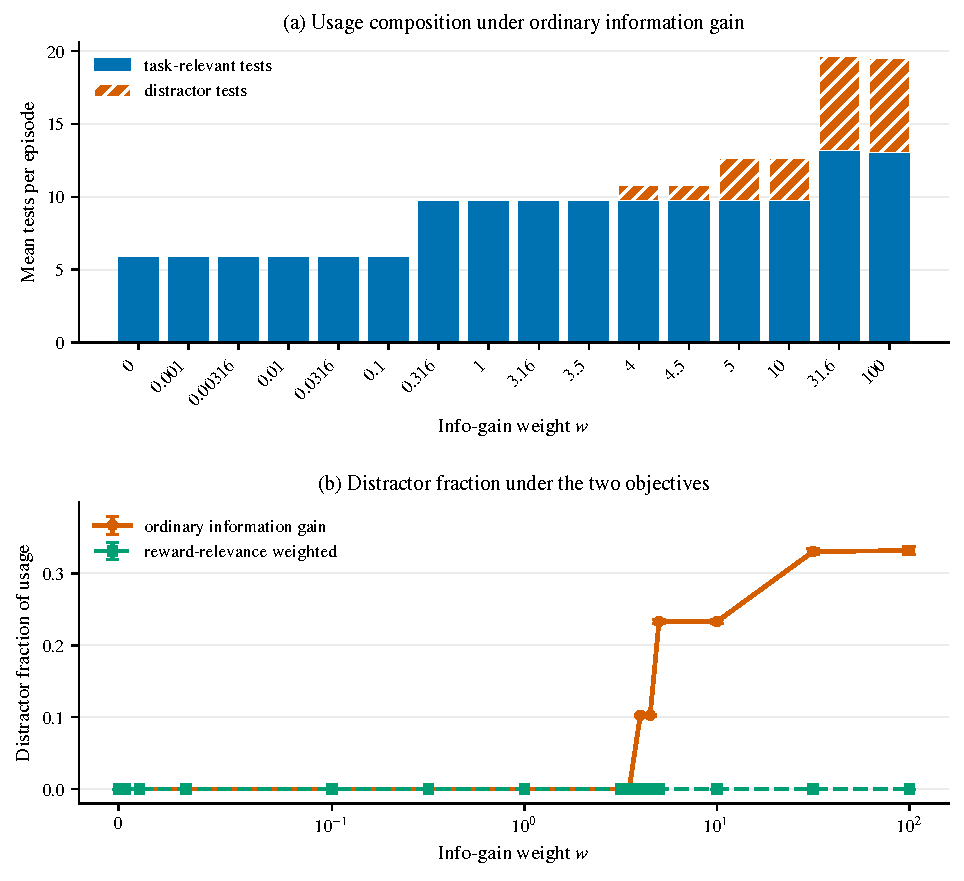
\includegraphics[width=\linewidth]{figures/distractor_composition.pdf}
\caption{Reward-irrelevant sensing on \texttt{DistractorDiagnosisEnv}. The upper panel decomposes ordinary Planning+IG's usage into task-relevant and distractor tests as $w$ grows. Distractor spend is zero below the onset bracket $(3.5, 4.0]$ and saturates at roughly a third of total usage. The lower panel plots the distractor fraction for ordinary information gain against the reward-relevance-weighted variant on the same grid. The weighted variant is flat at exactly zero everywhere. Error bars are seed-level SE over 5 seeds.}
\label{fig:distractor}
\Description{Two vertically stacked panels. The upper panel is a stacked bar chart of mean tests per episode across sixteen weight values, with blue task-relevant segments stepping from about 6 up to about 13 and a vermillion distractor segment that is absent at small weights, first appears at a weight of 4, and grows the stack to about 20 tests at the two largest weights. The lower panel plots two curves of distractor fraction against weight on a symmetric-log axis, linear near zero. The vermillion curve for ordinary information gain is flat at zero up to a weight of 3.5, rises steeply from 0.10 at weight 4 through 0.23 at weight 5, and levels off near 0.33. The green curve for the reward-relevance-weighted variant lies flat on zero across the entire range.}
\end{figure}

\subsection{Additional Onset and Operating-Point Checks}
\label{sec:budget_breadth_summary}

Positive-threshold two-state instances place the observed onset within one refined grid step, $3\%$, above the closed-form threshold, while standard negative-threshold instances observe already at $w{=}0$ (Appendix~\ref{sec:prop2exp}). The atlas collects the implicit $w{=}1$ budgets and two grid brackets per instance from the measured curves (Appendix~\ref{app:w_atlas}). These are measured operating points, not a universal predictive formula for the price.

\section{Results}
\label{sec:results}

The second battery locates the canonical EFE weight within the policy family and compares it with other planners. It provides empirical context for the equivalence result, whose validity itself rests on the stated assumptions and proof. We retain the main comparisons here and place detailed per-environment mechanisms, robustness studies, and additional tables in Appendix~\ref{app:extended_efe_results}.

\subsection{Core Environments}

Table~\ref{tab:main} contrasts $w{=}1$ EFE with myopic reward maximization, same-horizon reward-only Planning, and Planning+IG tuned for success within its own class. Reward-maximizing weights are considered separately below. On Tiger, EFE and Planning produce identical trajectories. With one observation action, the information term never changes the reward-based action choice at these stakes. This is a measured property of this instance rather than a general consequence of having a single sensor.

\begin{table}[ht]
\centering
\caption{Core comparison, $1{,}000$ episodes per seed over five seeds. Reward is mean $\pm$ seed-level SE. Here $w^*=w^*_{\mathrm{succ}}$ is tuned for success, with reward tuning reported separately. Bold identifies EFE and its exact Tiger tie with Planning, not a per-column winner. Success-tuned Planning+IG buys greater accuracy at a reward cost. Full agents, pooled uncertainties, and statistical comparisons are in Appendices~\ref{app:full_tables} and~\ref{app:stats}.}
\label{tab:main}
%% Numbers in this table are produced by experiments/run_experiment.py all
\begin{tablebody}
\begin{tabular}{llccc}
\toprule
Environment & Agent & Obs. & Success & Reward \\
\midrule
\multirow{4}{*}{\shortstack[l]{Tiger\\[-1pt]{\tablefontsize $H{=}6,\;w^*{=}50$}}} & Myopic & $1.00$ & 85.3\% & $-7.15 \pm 0.41$ \\
& \textbf{Planning} & $\mathbf{4.20}$ & $\mathbf{99.4\%}$ & $\mathbf{+5.19 \pm 0.21}$ \\
& Planning+IG & $5.66$ & 99.9\% & $+4.21 \pm 0.08$ \\
& \textbf{EFE} & $\mathbf{4.20}$ & $\mathbf{99.4\%}$ & $\mathbf{+5.19 \pm 0.21}$ \\
\midrule
\multirow{4}{*}{\shortstack[l]{Diagnosis\\[-1pt]{\tablefontsize $H{=}3,\;w^*{=}50$}}} & Myopic & $2.00$ & 64.7\% & $-13.17 \pm 0.58$ \\
& Planning & $5.86$ & 88.8\% & $-2.57 \pm 0.20$ \\
& Planning+IG & $13.16$ & 99.2\% & $-3.66 \pm 0.12$ \\
& \textbf{EFE} & $\mathbf{9.66}$ & $\mathbf{97.2\%}$ & $\mathbf{-1.37 \pm 0.18}$ \\
\midrule
\multirow{4}{*}{\shortstack[l]{Bandit\\[-1pt]{\tablefontsize $H{=}2,\;w^*{=}20$}}} & Myopic & $2.06$ & 62.2\% & $+5.56 \pm 0.09$ \\
& Planning & $3.29$ & 71.0\% & $+5.75 \pm 0.08$ \\
& Planning+IG & $9.57$ & 98.9\% & $+5.11 \pm 0.04$ \\
& \textbf{EFE} & $\mathbf{5.11}$ & $\mathbf{86.9\%}$ & $\mathbf{+6.27 \pm 0.04}$ \\
\bottomrule
\end{tabular}
\end{tablebody}
\end{table}

On Diagnosis, EFE raises success from $88.8\%$ to $97.2\%$ relative to Planning and improves reward from $-2.57$ to $-1.37$. Seed-level Welch tests give $p=4.0{\times}10^{-8}$ for success and $p=0.002$ for reward. On Bandit it raises success from $71.0\%$ to $86.9\%$ and reward from $5.75$ to $6.27$, with $p=2.1{\times}10^{-5}$ and $p=0.001$. These differences survive the stated Holm correction. Thus EFE Pareto-dominates same-horizon reward-only Planning on these two environments. Success-tuned Planning+IG reaches higher accuracy, $99.2\%$ and $98.9\%$, but pays for more sensing and attains lower reward. EFE supplies an untuned trade-off, not the best value of every metric.

Two baselines limit any attribution of these outcomes solely to explicit information gain. Posterior-vote, which draws states from the belief and votes over their optimal actions without an information term, is not significantly different from EFE on any Bandit metric. Its reward is nominally higher, $6.32$ against $6.27$ ($p=0.58$). It also beats EFE on Testbed, but performs worse on Diagnosis and Tiger. The Epistemic-only ablation commits immediately at chance-level success on all three core environments and Tileworld. Removing the pragmatic term therefore causes degenerate non-exploration in this implementation. Full baselines, pooled effect sizes, and seed-level tests appear in Appendices~\ref{app:full_tables}, \ref{app:stats}, and~\ref{app:core_details}. Reward effects against Planning are small at the episode level on Diagnosis and Bandit despite statistically detectable mean differences. We do not interpret the mechanically inflated effect sizes computed from only five seed means.

POMCP provides a search-based comparison, reported in Appendix~\ref{app:pomcp}. Its simulation count per decision is a computational budget distinct from the sensing budget $B$. The MCTS-EFE comparison matches simulation counts, while a separate Tiger control matches wall-clock computation. The original POMCP comparisons use untuned exploration constants. A separate sweep selects constants on tuning seeds under a recorded rule, but the canonical five-seed sweep had already been inspected before that rule was written. The Tiger tuning result is therefore retrospective. Neither the POMCP comparison nor the component ablation isolates directed observation selection as the cause of every performance difference. These qualifications remain necessary when comparing search architectures, even when the information-weighted family performs well.

\subsection{Where the Information-Unit Weight Sits}
\label{sec:pareto}

We sweep $w\in\{0.01,0.1,0.5,1,2,5,10,20,50,100,200\}$ on Tiger, Diagnosis, Bandit, Testbed, and Tileworld. Figure~\ref{fig:pareto} shows reward against success. The $w{=}1$ Planning+IG and EFE markers coincide under Proposition~\ref{prop:equivalence} and shared tie-breaking. The empirical question is where that common policy lies relative to other weights, not whether equivalent implementations differ.

\begin{figure}[tbp]
\centering
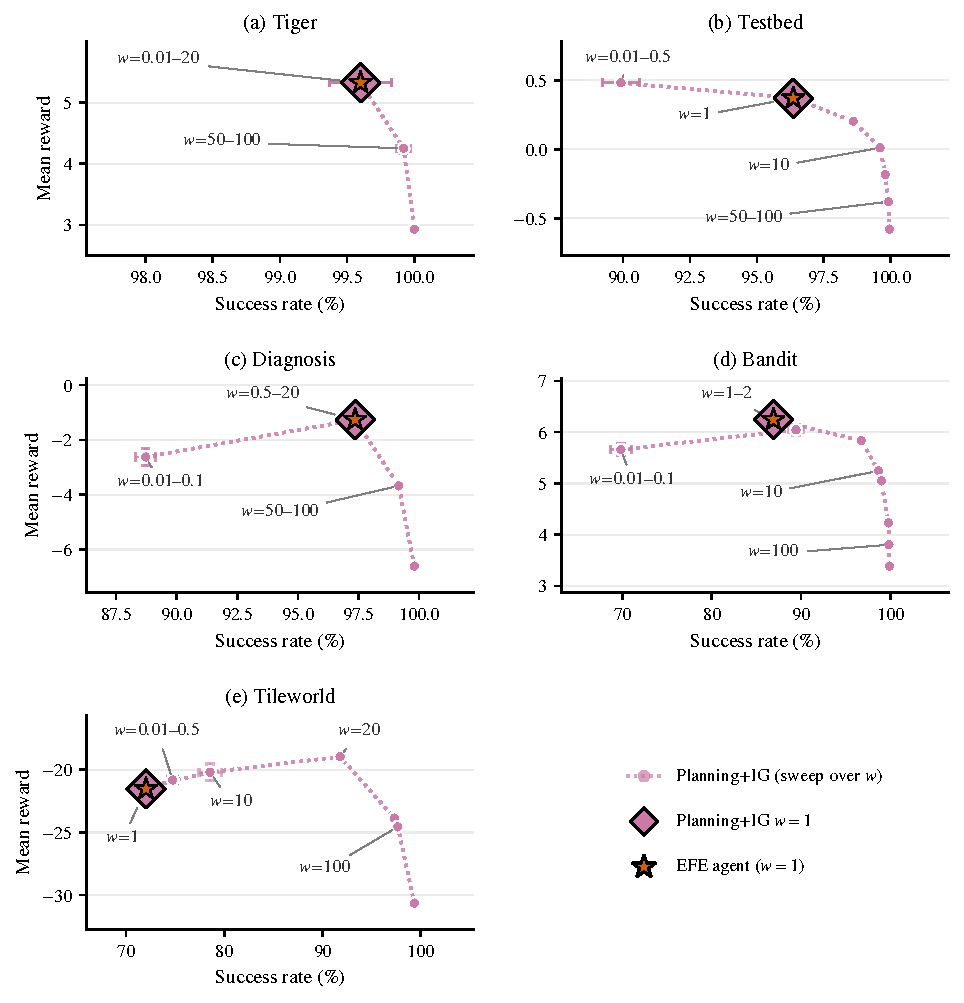
\includegraphics[width=\linewidth]{figures/fig_pareto.pdf}
\caption{Reward and success across eleven information weights from $0.01$ to $200$. The $w{=}1$ Planning+IG diamond and EFE star coincide under their equivalence assumptions and shared tie-breaking. They attain the largest sampled mean reward on Tiger, Diagnosis, and Bandit. On Testbed they trade reward for success, and on Tileworld $w{=}20$ dominates them on both axes. Labels identify sampled weights sharing a point. Error bars are seed-level SE, visible where larger than markers.}
\label{fig:pareto}
\Description{Five line plots arranged in a three by two grid, one per environment (Tiger, Testbed, Diagnosis, Bandit, Tileworld), with the legend in the sixth cell, each tracing mean reward against success rate as a pink dotted curve of connected dots swept over the info-gain weight, with weight labels in empty regions connected to their points by thin leaders, several as tied ranges such as w equals 0.01 to 20, and seed-level error bars visible on the lowest-success points. On Diagnosis, Bandit, and Tileworld the curve rises to a knee and then bends sharply downward as success approaches 100 percent, while on Tiger and Testbed the curve only descends as success rises. A large pink diamond with a vermillion star inside sits on each curve, at the reward peak in the Tiger, Diagnosis, and Bandit panels, partway down the descent in the Testbed panel, and clearly down and to the left of the w equals 20 knee in the Tileworld panel.}
\end{figure}

The weight-one policy is within the reward-maximizing run of sampled weights on Tiger ($0.01$ through $20$), Diagnosis ($0.5$ through $20$), and Bandit ($1$ and $2$). These are sampled plateaus, not claims about every untested weight between grid points. Testbed instead maximizes reward across sampled weights from $0.01$ through $0.5$. Its weight-one policy buys $6.4$ percentage points of success at a reward cost of $0.11$. On Tileworld, $w{=}20$ Pareto-dominates $w{=}1$, with reward $-18.95$ against $-21.53$ and success $91.8\%$ against $72.0\%$. Thus the canonical weight attains the sampled reward maximum on three of five environments and is suboptimal on two.

Success favors larger weights throughout this sweep, with its maximum at the upper grid endpoint $200$ on all five environments. The reward cost need not grow smoothly. On Tiger and Diagnosis, the tested weights from $1$ up to the point below $50$ leave reward unchanged, and the step to $50$ incurs the measured cost. The grid does not exclude a cheaper untested intermediate policy. The advantage of $w{=}1$ here is that it selects a useful default without environment-specific search under the stated reward convention. It does not remove dependence on units, promise best accuracy, or replace calibration when a particular sensing target is required. Appendix~\ref{app:pareto_details} retains the detailed trade-offs, and Appendix~\ref{app:nat_canonical} compares the implementation's bit-unit default with the exactly nat-canonical weight.

\subsection{Tileworld}
\label{sec:tileworld}

Tileworld shows why horizon and observation structure must accompany a scaling claim. At $6{\times}6$ and $H{=}2$, EFE and Planning are not significantly different in reward ($-21.53$ against $-21.39$, $p=0.82$) or success ($72.0\%$ against $73.8\%$, $p=0.17$). EFE uses fewer scans, $14.75$ against $15.64$ ($p=8.8{\times}10^{-5}$). These are failures to reject reward and success differences, not TOST equivalence. The success-tuned $w{=}50$ agent reaches $97.3\%$ accuracy but uses $32.25$ scans and earns lower reward. Table~\ref{tab:tileworld} and Figure~\ref{fig:tw_comparison} retain the full comparison and an illustrative trajectory in Appendix~\ref{app:tileworld_details}.

In a separate fixed-$H{=}2$ sweep (Figure~\ref{fig:tw_scaling}), Planning takes no scans at $8{\times}8$ and achieves $1.4\%\pm0.3$ percentage points success, while EFE achieves $69.4\%\pm1.0$. The short horizon cannot value enough scans to repay their costs before committing on a large grid. The contrast is therefore with a non-scanning finite-horizon agent, not with reward-only planning at arbitrary depth. At $4{\times}4$ and $6{\times}6$ the two are within one SE, with no formal test for that sweep. The advantage appears at a horizon-and-scale threshold rather than widening uniformly with size. Its weighted comparators use fixed $w{=}100$, not class-specific tuning. Random and overlapping scan partitions sharply reduce all agents' absolute performance and do not separate EFE from Planning on reward or success, although EFE uses fewer scans in all three modes. Appendix~\ref{app:tileworld_details} preserves these robustness results and their scope.

\begin{figure}[tbp]
\centering
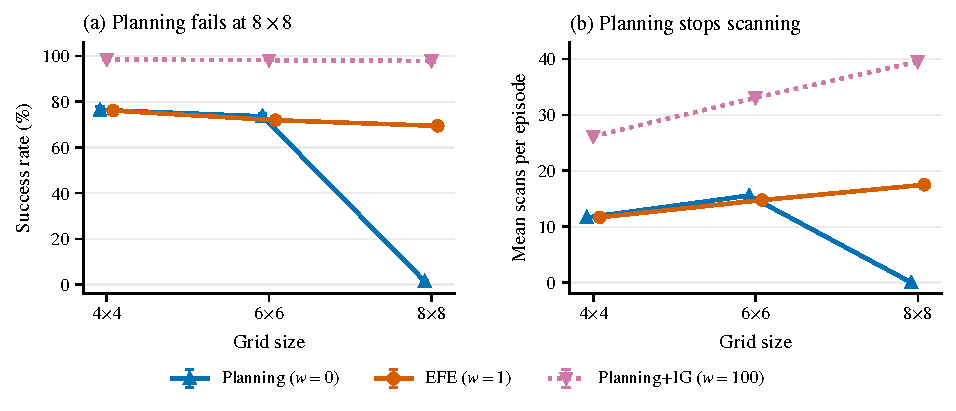
\includegraphics[width=\linewidth]{figures/fig_tileworld_scaling.pdf}
\caption{Tileworld scaling ($H{=}2$, 200 episodes per seed $\times$ 5 seeds) across Myopic, Planning, InfoGain-Tuned, Planning+IG, and EFE. Planning collapses at $8{\times}8$ ($|S|{=}64$), while EFE maintains $69.4\%$. Planning+IG at a fixed $w{=}100$, not tuned in class, achieves $97.8\%$ but at higher reward cost. Error bars in (a) and (b) are seed-level SE, tied series are offset slightly along the categorical axis for legibility, and per-episode time in (c) is a pooled mean over all episodes and seeds, shown without error bars on a log scale.}
\label{fig:tw_scaling}
\Description{Three line plots against grid sizes 4 by 4, 6 by 6, and 8 by 8. The left panel shows success rate, where the pink dotted Planning+IG and orange InfoGain-Tuned lines stay near 100 percent, the vermillion EFE line declines gently from about 76 to about 69 percent, the blue Planning line drops from about 76 percent to near zero at the largest grid, and the gray dashed Myopic line falls from about 40 percent to near zero by 6 by 6. The middle panel shows mean reward declining for all agents as grids grow, with the vermillion line ending highest near minus 26 and the blue and gray lines ending near minus 49. The right panel shows per-episode computation time on a log scale, where the pink line is highest and ends near 890 milliseconds, the vermillion line is next near 400 milliseconds, the orange line sits near 70 milliseconds, the blue line peaks near 40 milliseconds at 6 by 6 before falling to a few milliseconds, and the gray line is lowest below one millisecond.}
\end{figure}

\subsection{RockSample}
\label{sec:rocksample}

RockSample tests the information weight within a shared factored belief-space search and a shared greedy leaf rule. On RS[5,3], EFE ($16.47$) and the $w{=}5$ comparator ($16.41$) are not significantly different. On RS[7,4], EFE earns $15.96$ against $14.56$ and leads the weighted family ($p<10^{-5}$). On RS[7,8], EFE ($21.85$) and $w{=}5$ ($23.76$) are not significantly different after correction, and both outperform reward-only Planning ($12.31$). Raising the weight from $5$ to $10$ significantly hurts on two of these instances and does not significantly help on the third. Only weights $1$, $5$, and $10$ were compared here, so this is not a dense reward-tuning claim.

\input{tables/rocksample_main.tex}

The important counterexample is RS[11,11]. EFE and Planning both earn $13.23$, while a standalone approach-then-check heuristic earns $28.66\pm0.83$. That heuristic also beats both weighted agents on RS[7,8]. Larger state space therefore does not itself increase the value of information weighting. At feasible search depths, distant useful checks lie beyond the tree, and the shared leaf rule values untouched rocks at zero under the uniform prior. It also charges a phantom trip to the east edge before exit, although this variant allows exit anywhere, biasing depth-capped continuations toward early exit. The cost is shared across the weighted family but limits absolute performance. Deeper POMCP does not repair this instance in the tested configurations. Behavioral traces show many distant checks, and reward declines from $12.94$ at horizon $10$ to $-54.78$ at horizon $40$. Table~\ref{tab:rocksample} gives the full comparison. Appendix~\ref{app:rocksample_main_details} retains the leaf-rule disclosure, depth check, and heuristic comparison, alongside the extended solver analysis in Appendix~\ref{app:rocksample}.

\subsection{Structural Inspection}
\label{sec:inspection}

Inspection makes the reward-accuracy trade-off explicit. At $N{=}8$, EFE improves accuracy from Planning's $73.0\%$ to $91.1\%$ while reward falls from $-17.85$ to $-20.95$. At $N{=}16$, it improves accuracy from $78.2\%$ to $90.8\%$, with reward $-45.80$ against $-45.42$, a non-significant difference ($p=0.57$). The $w{=}5$ agent attains higher accuracy, $97.3\%$, but uses $38.3$ tests against EFE's $28.1$ and earns $-54.74$. These results demonstrate feasible factored search on a synthetic known-model problem with a hand-coded leaf rule. They do not validate industrial deployment or show that EFE uniquely optimizes either reward or accuracy. Table~\ref{tab:inspection} reports both instances, with the qualified two-state interpretation in Appendix~\ref{app:inspection_details}.

\begin{table}[ht]
\centering
\caption{Structural Inspection results. $N{=}8$ and $N{=}16$ run 2{,}500 episodes each (500 per seed $\times$ 5 seeds). Reward and accuracy are reported as mean $\pm$ seed-level SE. Greedy diagnoses without testing. Bold marks the best accuracy and the best reward per instance, plus any value within sampling error of that best (seed-level Welch $p > 0.05$, uncorrected). The two are not always the same agent. EFE is a competitive untuned trade-off, not uniquely best on all metrics. Accuracy is the fraction of components correctly diagnosed.}
\label{tab:inspection}
%% Numbers in this table are produced by experiments/run_inspection.py
\begin{tablebody}
\begin{tabular}{llcccc}
\toprule
Instance & Agent & Accuracy & Missed & Tests & Reward \\
\midrule
\multirow{4}{*}{\shortstack[l]{$N{=}8$\\[-1pt]{\tablefontsize $|S|{=}256$}}} & Greedy & $70.7 \pm 0.5\%$ & $2.34$ & $0.0$ & $-114.33 \pm 1.96$ \\
& Planning ($w{=}0$) & $73.0 \pm 0.3\%$ & $0.07$ & $12.7$ & $\mathbf{-17.85 \pm 0.23}$ \\
& Planning+IG ($w{=}5$) & $\mathbf{96.3 \pm 0.1\%}$ & $0.10$ & $19.7$ & $-27.98 \pm 0.44$ \\
& EFE ($w{=}1$) & $91.1 \pm 0.2\%$ & $0.09$ & $15.5$ & $-20.95 \pm 0.30$ \\
\midrule
\multirow{4}{*}{\shortstack[l]{$N{=}16$\\[-1pt]{\tablefontsize $|S|{=}65{,}536$}}} & Greedy & $70.5 \pm 0.4\%$ & $4.72$ & $0.0$ & $-233.09 \pm 3.13$ \\
& Planning ($w{=}0$) & $78.2 \pm 0.2\%$ & $0.24$ & $22.4$ & $\mathbf{-45.42 \pm 0.23}$ \\
& Planning+IG ($w{=}5$) & $\mathbf{97.3 \pm 0.0\%}$ & $0.14$ & $38.3$ & $-54.74 \pm 0.40$ \\
& EFE ($w{=}1$) & $90.8 \pm 0.1\%$ & $0.24$ & $28.1$ & $\mathbf{-45.80 \pm 0.60}$ \\
\bottomrule
\end{tabular}
\end{tablebody}
\end{table}

Across the battery, the canonical weight is useful when the reward-only policy leaves valuable, representable sensing opportunities unused. Its benefit is bounded by the search horizon, sensor structure, reward convention, and objective of the comparison. It matches the sampled reward maximum on three of five swept environments, loses to other weights on two, and gains nothing over Planning on the largest RockSample instance. These limits matter alongside its positive results on Diagnosis, Bandit, and the largest fixed-horizon Tileworld grid.
